\documentclass[10pt,letterpaper,twocolumn]{article}

\usepackage[letterpaper,top=0.56in,bottom=0.58in,left=0.62in,right=0.62in,columnsep=0.20in]{geometry}
\usepackage{mathptmx}
\usepackage{microtype}
\usepackage{graphicx}
\usepackage{amsmath,amssymb}
\usepackage{booktabs}
\usepackage{array}
\usepackage{cite}
\usepackage{url}
\usepackage[hidelinks]{hyperref}
\usepackage[font=footnotesize,labelfont=bf,labelsep=period]{caption}
\usepackage{titlesec}
\usepackage{balance}
\usepackage{dblfloatfix}
\usepackage{placeins}

\graphicspath{{figures/}}
\setlength{\parindent}{1em}
\setlength{\parskip}{0pt}
\setlength{\columnsep}{0.20in}
\setlength{\textfloatsep}{6pt plus 1pt minus 1pt}
\setlength{\floatsep}{6pt plus 1pt minus 1pt}
\setlength{\intextsep}{5pt plus 1pt minus 1pt}
\setlength{\abovecaptionskip}{3pt}
\setlength{\belowcaptionskip}{-1pt}
\setlength{\tabcolsep}{3.0pt}
\renewcommand{\arraystretch}{1.06}
\renewcommand{\baselinestretch}{0.965}

\titleformat{\section}{\centering\scshape\fontsize{9.2}{10.2}\selectfont}{\Roman{section}.}{0.42em}{}
\titleformat{\subsection}{\itshape\fontsize{9.0}{10.0}\selectfont}{\Alph{subsection}.}{0.35em}{}
\titlespacing*{\section}{0pt}{5pt}{2.5pt}
\titlespacing*{\subsection}{0pt}{3.5pt}{1.5pt}

\newcommand{\Nzero}{$N0$}
\newcommand{\Nmid}{$N75$}
\newcommand{\Nfull}{$N_{\mathrm{Full}}$}
\newcommand{\method}{RMOF-Net}

\hypersetup{
  pdftitle={RMOF-Net for Maize Nitrogen Deficiency Detection and Treatment-Level Classification},
  pdfauthor={Xicheng Peng, Tao Zhong, Houjun Liu, Zixuan Shao, and He Zhu},
  pdfsubject={COMP9444 project summary report},
  pdfkeywords={maize nitrogen deficiency, RGB imaging, ordinal classification, cross-attention}
}

\title{\vspace{-0.25in}\bfseries 08--RMOF-Net for Maize Nitrogen Deficiency\\[-1pt]
Detection and Treatment-Level Classification\vspace{-0.08in}}
\author{\normalsize Xicheng Peng, Tao Zhong, Houjun Liu, Zixuan Shao, and He Zhu\\[-1pt]
\small z5526784, z5643577, z5461152, z5663409, z5696771}
\date{}

\begin{document}
\maketitle
\vspace{-0.22in}

\begin{abstract}
Nitrogen deficiency reduces maize productivity, whereas excess fertilisation increases economic and environmental cost. This paper considers field-RGB recognition as binary deficiency screening and three-level classification of \Nzero, \Nmid, and \Nfull treatments. We compare ImageNet-pretrained ResNet18, EfficientNet-B0, and DeiT-Tiny with the proposed Region-aware Multi-scale Ordinal Fusion Network (\method). \method{} combines global and $2\!\times\!2$ regional CNN features, regional colour statistics, learned colour texture, and region-wise cross-attention. Classification and ordinal-score heads are optimised jointly. On the 200-image test evaluation, full \method{} obtains 0.715 accuracy, 0.715 Macro-F1, 0.890 deficiency F1, and 0.310 ordinal MAE with 4.314M parameters. Compared with EfficientNet-B0, it improves Macro-F1 by 0.130 and reduces ordinal MAE by 42.1\%. It produces 143/200 correct predictions and five endpoint reversals, compared with 117/200 and 24 for the base model.
\end{abstract}

\noindent\textbf{Index Terms---}maize nitrogen deficiency, RGB imaging, ordinal classification, multi-scale features, cross-attention, precision agriculture.

\section{Introduction}

Nitrogen management requires balancing crop demand against fertiliser cost and environmental loss. Laboratory assays and manual scouting do not scale readily, whereas RGB imagery is inexpensive to acquire. However, field images contain soil, residue, weeds, shadows, and exposure variation that may correlate with treatment. In addition, chlorosis may occur in a limited leaf region. A global representation can attenuate these local symptoms, while a colour-only model may respond to illumination or background rather than nitrogen treatment.

For a class-probability vector $p=[p_0,p_1,p_2]$, the deficiency probability is $p_{\mathrm{def}}=p_0+p_1$, while the reported binary label is $\hat d=\mathbf{1}\{\hat y\in\{0,1\}\}$. The ordered treatment label uses $y\in\{0,1,2\}$ for \Nzero, \Nmid, and \Nfull, respectively. The task is image classification; the dataset does not provide boxes or symptom masks. \method{} uses two CNN depths, regional colour statistics, a learnable colour-texture encoder, region-wise cross-attention, and joint categorical--ordinal supervision. Evaluation includes class-wise performance, \Nzero$\leftrightarrow$\Nfull{} endpoint errors, and inference cost in addition to aggregate accuracy.

\section{Related Work}

CNNs have been applied to crop nutrient-stress recognition \cite{sethy2020,salaic2023}, although background content and acquisition shift remain important sources of error \cite{mohanty2016,plantdoc2020,mvmatch2024}. ResNet18 and EfficientNet-B0 are compact hierarchical CNN baselines \cite{resnet2016,efficientnet2019}, while DeiT-Tiny provides a compact transformer baseline \cite{deit2021}. RGB indices such as Excess Green provide interpretable plant cues \cite{woebbecke1995,meyer2008}, but their response can vary with illumination. \method{} combines such statistics with learned texture and uses cross-attention to match regional deep and colour evidence, extending scalar multimodal gating \cite{arevalo2017}. Squared Earth Mover's Distance (EMD) provides an ordered loss for the treatment labels \cite{hou2016}.

\section{Task and Dataset}

The public maize dataset contains 1,200 field-canopy images: 400 each for \Nzero, \Nmid{} (75 kg N/ha), and \Nfull{} (136 kg N/ha), spanning 238 genotypes \cite{salaic2023}. Images were acquired around flowering with a tripod-mounted DSLR at a $45^\circ$ angle. The fixed 200-image test split contains 70/60/70 images from the three classes. Related views and detected near-duplicates are kept within one partition; validation data from the remaining images is used only for model selection. The ordinal target $s=y\in\{0,1,2\}$ represents application-level order and is not a tissue-nitrogen, SPAD, yield, or calibrated physiological measurement.

\begin{figure*}[!t]
  \centering
  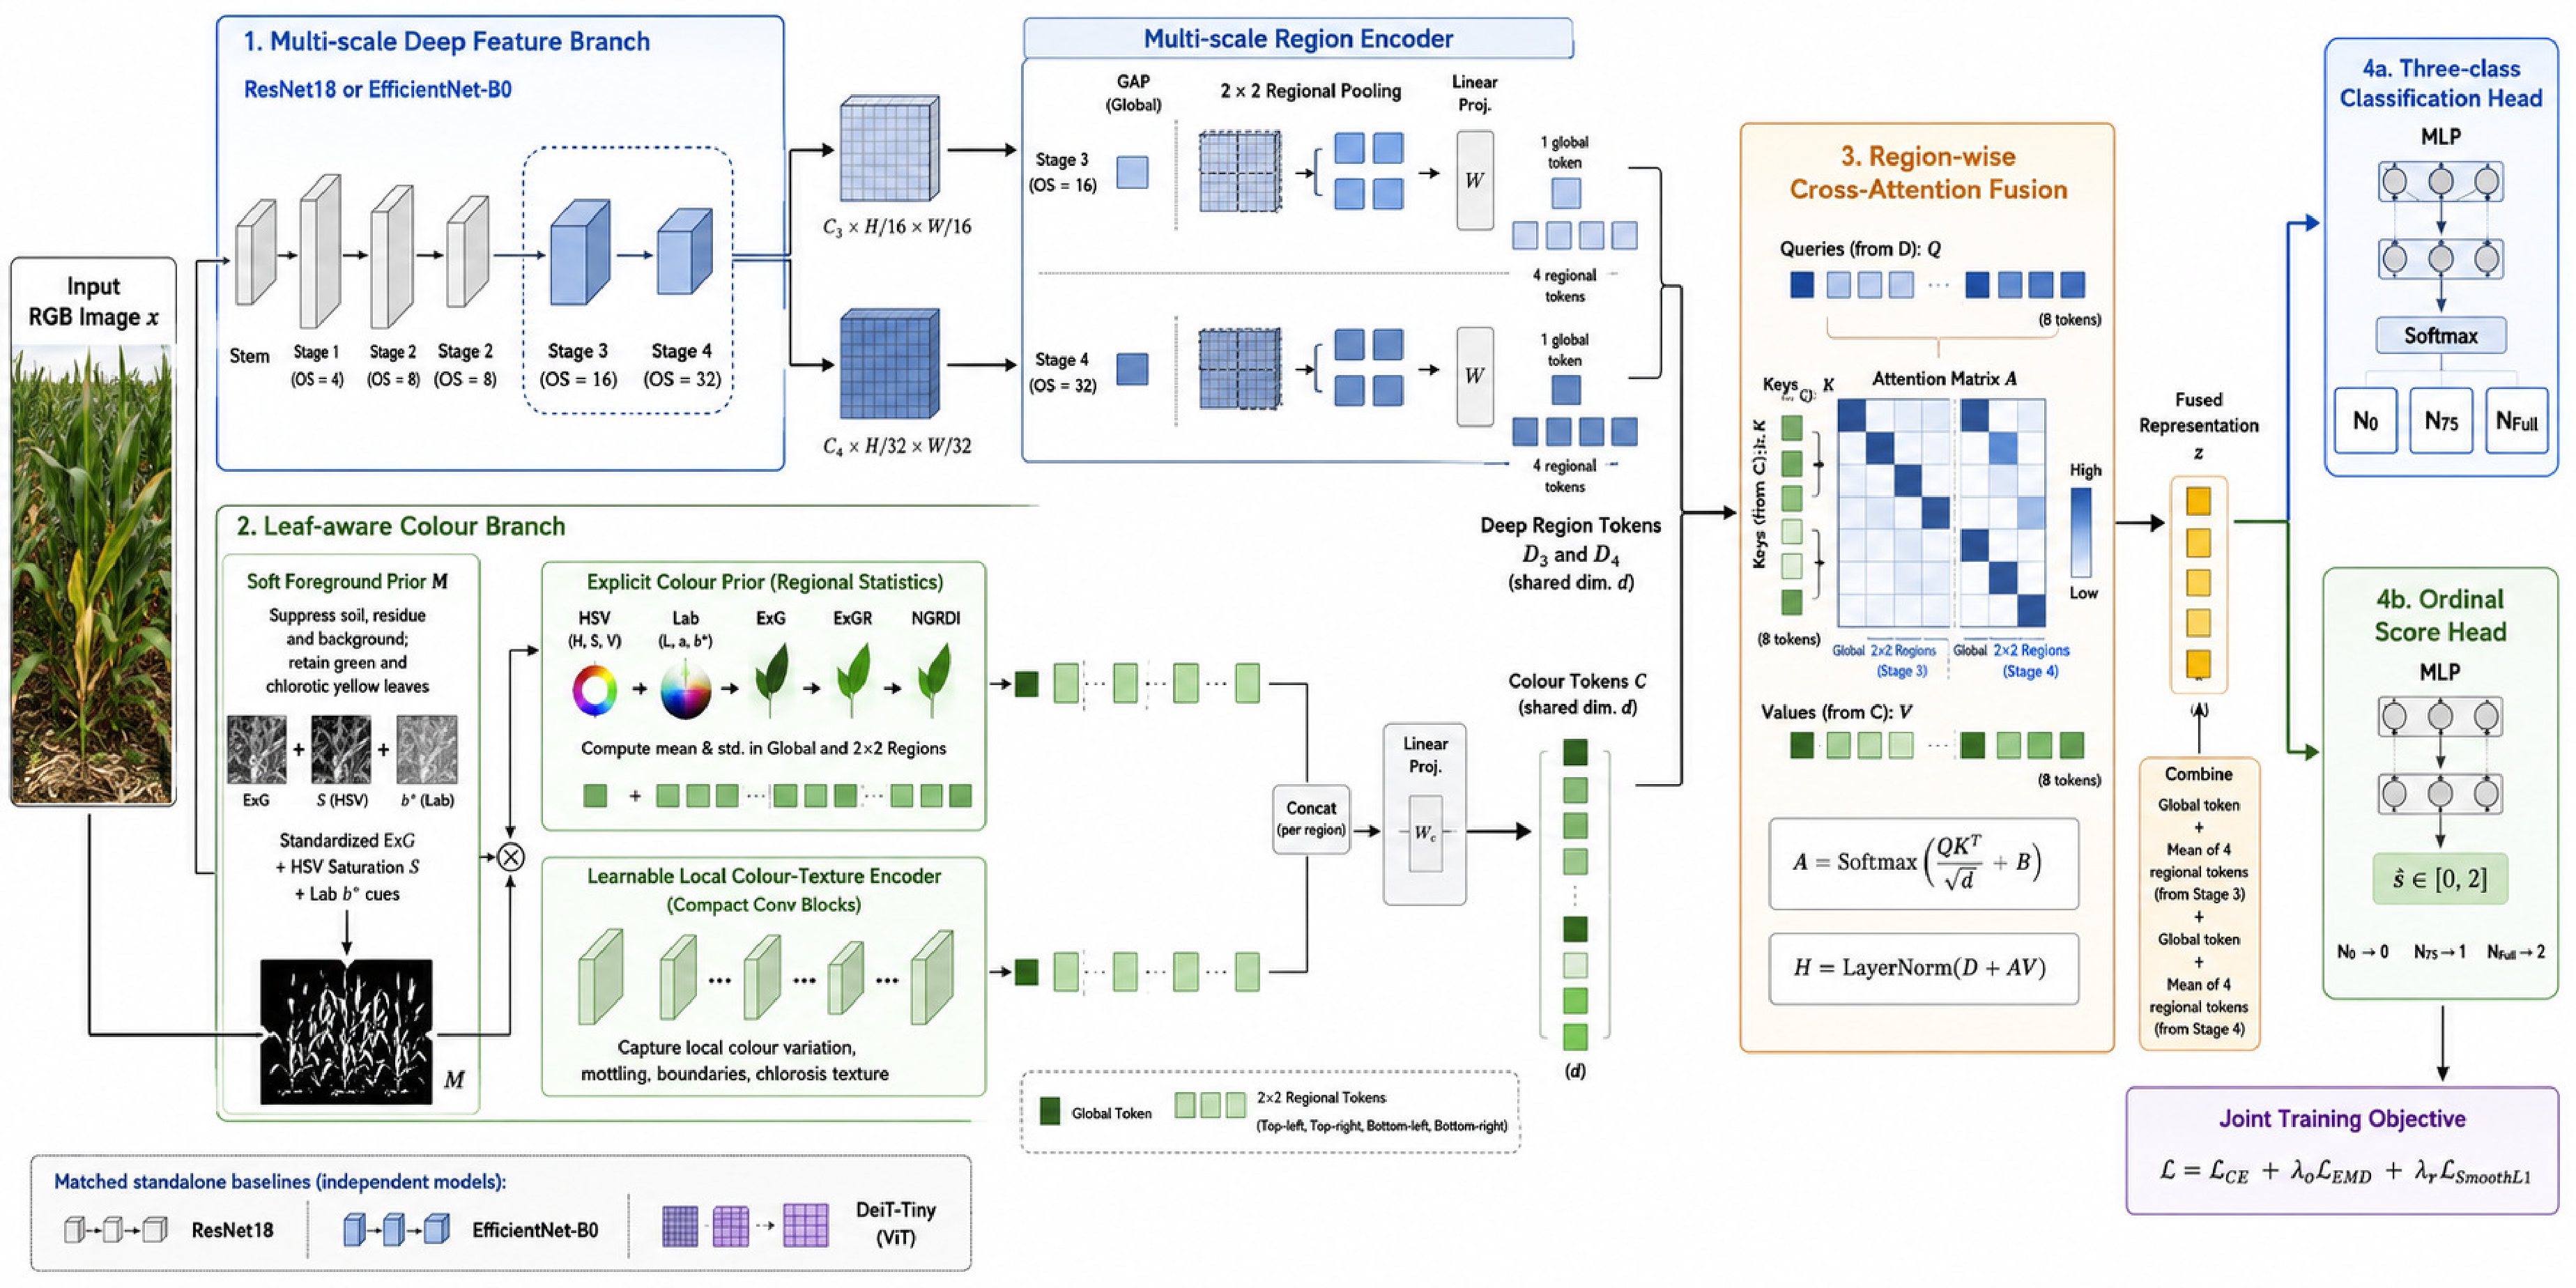
\includegraphics[width=0.92\textwidth]{figure1_rmof_overview.pdf}
  \caption{Overview of \method. A hierarchical CNN produces global and $2\!\times\!2$ regional features at two depths. A leaf-aware branch extracts region-aligned explicit colour priors and learned texture. Cross-attention forms a shared representation for treatment classification and ordinal-score prediction. ResNet18, EfficientNet-B0, and DeiT-Tiny are evaluated as matched standalone baselines.}
  \label{fig:overview}
\end{figure*}

\section{RMOF-Net}

\subsection{Inputs, backbone, and aligned regions}

Figure~\ref{fig:overview} summarises the model pipeline. Given an RGB image $x$, the selected hierarchical CNN (ResNet18 or EfficientNet-B0) produces Stage-3 and Stage-4 feature maps $F_3,F_4$ at output strides 16 and 32. The former retains fine chlorotic and mottled patterns; the latter represents broader canopy context. At each scale $l\in\{3,4\}$, adaptive pooling generates one global token and four regional tokens over the top-left, top-right, bottom-left, and bottom-right cells:
\begin{equation}
D_l=P_l[\operatorname{GAP}(F_l);\operatorname{RP}_{2\times2}(F_l)]\in\mathbb{R}^{5\times d}.
\label{eq:deep}
\end{equation}
The learned projection $P_l$ maps both scales to width $d$. Token $r=0$ represents the entire image and $r=1,\ldots,4$ represent the four cells in a fixed order. The colour stream uses the same ordering, which defines a correspondence between deep and colour regions. DeiT-Tiny is retained as a matched standalone baseline because its token hierarchy does not provide analogous Stage-3/Stage-4 CNN maps.

\subsection{Leaf-aware colour encoding}

The colour stream retains explicit chromatic evidence before fusion. For normalised RGB channels $R,G,B\in[0,1]$, its vegetation indices are
\begin{equation}
\begin{aligned}
\mathrm{ExG}&=2G-R-B, & \mathrm{ExGR}&=3G-2.4R-B,\\[-2pt]
\mathrm{NGRDI}&=\frac{G-R}{G+R+\epsilon},
\end{aligned}
\label{eq:indices}
\end{equation}
where $\epsilon>0$ prevents division by zero. Each scalar cue $v$ is standardised with training-set statistics, $\widetilde v=(v-\mu_v)/(\sigma_v+\epsilon)$, and $\operatorname{LSE}(v_1,\ldots,v_m)=\log\sum_{i=1}^{m}\exp(v_i)$. A soft foreground prior then suppresses soil and residue while retaining yellow leaves: $u=\operatorname{LSE}(\widetilde{\mathrm{ExG}},\widetilde S,\widetilde b^{*})$ and $m=\sigma(\gamma(u-\tau))$. Here $\tau$ is fitted without test images and $\gamma>0$ controls the transition width, so $m$ assigns continuous rather than binary foreground weights.

Let $\mathcal H=\{H,S,V,L^*,a^*,b^*,\mathrm{ExG},\mathrm{ExGR},\mathrm{NGRDI}\}$. For the global region and each $2\!\times\!2$ cell, the statistic descriptor is $a_r=\operatorname{concat}_{h\in\mathcal H}[\mu_r(h),\sigma_r(h)]$. A shallow convolutional encoder $\phi$ processes the masked image $x\odot m$ to obtain local texture. Both components are pooled by the same regional operator and projected to a colour token:
\begin{equation}
t_r=\operatorname{Pool}_r(\phi(x\odot m)),\qquad C_r=W_c[a_r;t_r].
\label{eq:colour}
\end{equation}
The resulting $C=[C_0,\ldots,C_4]\in\mathbb{R}^{5\times d}$ has the same global--regional layout as $D_l$. The explicit component encodes regional chromatic summaries; $t_r$ represents boundaries, mottling, and local chlorosis not described by the fixed indices.

\subsection{Region-wise fusion and ordered learning}

At each scale, the deep tokens attend to the five colour tokens. With $Q_l=D_lW_l^Q$, $K=CW^K$, $V=CW^V$, and $B_l\in\mathbb{R}^{5\times5}$, the row-wise attention and residual update are
\begin{equation}
\begin{aligned}
A_l&=\operatorname{softmax}\!\left(\frac{Q_lK^\top}{\sqrt d}+B_l\right),\\[-2pt]
H_l&=\operatorname{LN}(D_l+A_lV).
\end{aligned}
\label{eq:attention}
\end{equation}
Each row $A_l[r,:]\in\mathbb{R}^{5}$ weights the colour regions for a deep query. The alignment bias $B_l$ favours the corresponding cell but does not constrain the attention to the diagonal. Thus, a local deep token may use global colour context or another region when the learned affinities support it. In contrast, the scalar-gate ablation applies one image-level fusion weight. Global and regional summaries from both scales are concatenated as
\begin{equation}
z=[H_{3,0};\tfrac14\sum_{r=1}^{4}H_{3,r};H_{4,0};\tfrac14\sum_{r=1}^{4}H_{4,r}]\in\mathbb{R}^{4d}.
\label{eq:aggregate}
\end{equation}
The classification head gives $p=\operatorname{softmax}(W_pz+b_p)$, and the ordinal head gives the continuous auxiliary score $\tilde{s}=2\sigma(w_s^\top z+b_s)\in[0,2]$. For one-hot target $q$ and $K=3$ classes, the ordered term compares cumulative distributions, $\mathcal L_{\mathrm{EMD}}=\frac{1}{K-1}\sum_{k=0}^{K-2}(\sum_{j=0}^{k}p_j-\sum_{j=0}^{k}q_j)^2$. The training objective is
\begin{equation}
\mathcal L=\mathcal L_{\mathrm{CE}}+\lambda_o\mathcal L_{\mathrm{EMD}}+
\lambda_r\operatorname{SmoothL1}(\tilde{s},s),
\label{eq:loss}
\end{equation}
where $\mathcal L_{\mathrm{CE}}=-\sum_{j=0}^{2}q_j\log p_j$, $\lambda_o,\lambda_r\geq0$ are validation-selected weights, and $\operatorname{SmoothL1}(\tilde{s},s)=\rho_1(\tilde{s}-s)$ with
\begin{equation}
\rho_1(e)=
\begin{cases}
\tfrac12e^2, & |e|<1,\\[-2pt]
|e|-\tfrac12, & \text{otherwise}.
\end{cases}
\label{eq:smoothl1}
\end{equation}
The cumulative EMD term assigns a larger penalty to endpoint confusions than to adjacent errors. At inference, $\hat y=\arg\max_jp_j$ is the reported treatment class; $\tilde{s}$ regularises the shared representation and provides a continuous ordered auxiliary output.

\section{Experimental Setup}

Inputs are resized to $224\!\times\!224$ and ImageNet-normalised \cite{imagenet2009}. Training uses horizontal flips, small rotations/crops, and mild brightness/contrast jitter. All trainable models receive the same split and tuning budget. Standard ImageNet-pretrained classifiers are optimised with AdamW and cosine decay \cite{adamw2019}; learning rate, weight decay, batch size, and dropout are validation-selected. The component ladder starts from EfficientNet-B0. The scalar-gate row is the direct fusion control; full \method{} replaces that gate with region-wise cross-attention and joint ordinal supervision.

Def.-F1 evaluates $\{N0,N75\}$ against \Nfull. Macro-F1 is the primary three-class score; we additionally report accuracy, class-wise F1, ordinal MAE, parameter count, and batch-one latency. The tabulated metric is $\mathrm{Ord\mbox{-}MAE}=n^{-1}\sum_{i=1}^{n}|\hat y_i-y_i|$. Thus Figure~\ref{fig:error} counts the same hard-label residuals $r_i=\hat y_i-y_i\in\{-2,-1,0,1,2\}$ that determine ordinal MAE. Latency uses the same accelerator, precision, input path, warm-up, and timing protocol. Repeated results are shown as mean$\pm$standard deviation where available; unadorned cells are point estimates from the controlled component study.

\begin{table*}[!t]
\centering
\caption{Main comparison and cumulative component analysis. The scalar gate is a direct-fusion control; full \method{} replaces it with region-wise cross-attention and ordinal supervision. Higher is better except Ord.-MAE, parameters, and latency.}
\label{tab:main}
\scriptsize
\resizebox{\textwidth}{!}{%
\begin{tabular}{lccccccccc}
\toprule
Method & Def.-F1$\uparrow$ & Acc.$\uparrow$ & Macro-F1$\uparrow$ & $F1_{N0}\uparrow$ & $F1_{N75}\uparrow$ & $F1_{N_{Full}}\uparrow$ & Ord.-MAE$\downarrow$ & Params (M)$\downarrow$ & Latency (ms/img)$\downarrow$ \\
\midrule
ResNet18 & $0.831\pm0.005$ & $0.619\pm0.033$ & $0.588\pm0.031$ & $0.777\pm0.020$ & $0.365\pm0.090$ & $0.624\pm0.088$ & $0.411\pm0.028$ & 11.178 & $0.690\pm0.003$ \\
DeiT-Tiny & $0.764\pm0.088$ & $0.515\pm0.057$ & $0.435\pm0.049$ & $0.659\pm0.038$ & $0.136\pm0.139$ & $0.512\pm0.212$ & $0.602\pm0.087$ & 5.525 & $0.795\pm0.017$ \\
EfficientNet-B0 (Base) & 0.788 & 0.585 & 0.585 & 0.627 & 0.563 & 0.565 & 0.535 & 4.011 & 0.555 \\
\quad + multi-scale regions & 0.825 & 0.612 & 0.606 & 0.762 & 0.410 & 0.645 & 0.420 & 4.069 & 0.565 \\
\quad + explicit colour priors & 0.818 & 0.605 & 0.594 & 0.755 & 0.395 & 0.632 & 0.435 & 4.073 & 0.994 \\
\quad + learned colour texture & 0.845 & 0.658 & 0.660 & 0.790 & 0.485 & 0.705 & 0.380 & 4.182 & 1.137 \\
\quad + scalar fusion gate & 0.855 & 0.672 & 0.680 & 0.805 & 0.510 & 0.725 & 0.365 & 4.214 & 1.137 \\
\textbf{Full \method} & \textbf{0.890} & \textbf{0.715} & \textbf{0.715} & \textbf{0.740} & \textbf{0.618} & \textbf{0.788} & \textbf{0.310} & 4.314 & 1.143 \\
\bottomrule
\end{tabular}}
\end{table*}

\section{Results and Discussion}

\subsection{Main comparison}

Table~\ref{tab:main} reports 0.715 accuracy, 0.715 Macro-F1, and 0.890 deficiency F1 for full \method{}. Relative to EfficientNet-B0, \Nmid{} F1 increases from 0.563 to 0.618, and both endpoint F1 values also improve. The ordinal MAE decreases from 0.535 to 0.310, indicating that incorrect predictions are, on average, closer to the ordered target.

ResNet18 is the strongest standalone baseline in Macro-F1 (0.588). Full \method{} exceeds it by 0.127 Macro-F1 and 0.096 accuracy while using 4.314M rather than 11.178M parameters. Relative to the EfficientNet-B0 starting point, the corresponding gains are 0.130 Macro-F1, 0.130 accuracy, and 0.102 deficiency F1. The component comparison therefore supports the use of regional colour information in addition to global CNN features.

\subsection{Ablation analysis}

Figure~\ref{fig:ablation} quantifies the contribution of each component. Adding multi-scale regions increases Macro-F1 from 0.585 to 0.606 and reduces MAE from 0.535 to 0.420, but it shifts performance toward the endpoint classes: $F1_{N75}$ falls from 0.563 to 0.410. The result suggests that the $2\!\times\!2$ decomposition retains useful spatial variation but does not, by itself, resolve the intermediate treatment. Adding explicit colour priors to this multi-scale configuration decreases Macro-F1 from 0.606 to 0.594 and increases MAE from 0.420 to 0.435, consistent with sensitivity of fixed colour statistics to illumination, residue, or exposure.

\begin{figure}[!t]
  \centering
  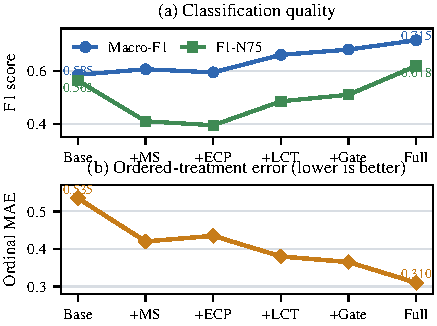
\includegraphics[width=0.94\columnwidth]{figure2_component_ablation.pdf}
  \caption{Component trends. MS: multi-scale regions; ECP: explicit colour priors; LCT: learned colour texture. The final configuration combines learned texture, region-wise fusion, and ordered supervision.}
  \label{fig:ablation}
\end{figure}

Adding learned colour texture produces the largest Macro-F1 increase in the component sequence, reaching 0.660 Macro-F1 and 0.485 \Nmid{} F1 while reducing MAE to 0.380. This branch can represent local boundaries, mottling, and chlorosis beyond fixed chromatic thresholds. The scalar gate yields a smaller additional improvement. Replacing it with region-wise cross-attention and ordinal supervision gives 0.715 Macro-F1, 0.618 \Nmid{} F1, and 0.310 MAE. These results indicate that learned local colour features are most useful when fused selectively with deep regional features.

\subsection{Error analysis}

Figure~\ref{fig:error} reports the fixed 200-image test split. Full \method{} increases the number of correct predictions from 117 to 143 and reduces \Nzero$\leftrightarrow$\Nfull{} reversals from 24 to five (79.2\%). The residual distribution contains 143 zero-residual predictions; 52 of the remaining 57 errors are adjacent treatment levels.

\begin{figure}[!t]
  \centering
  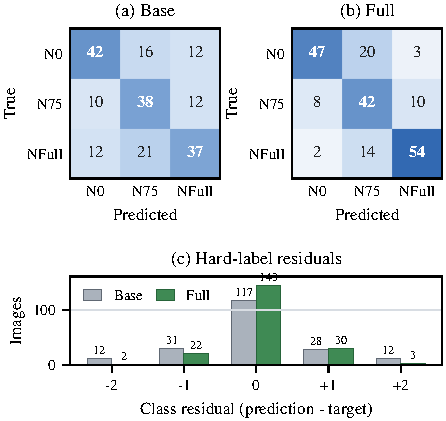
\includegraphics[width=0.95\columnwidth]{figure3_error_analysis.pdf}
  \caption{Single-column error analysis on the 200-image test split. (a--b) Confusion matrices; (c) hard-label residuals $r=\hat y-y$. Residuals of $\pm2$ are severe \Nzero$\leftrightarrow$\Nfull{} reversals.}
  \label{fig:error}
\end{figure}

The confusion matrices identify the source of this change. For true \Nfull{}, correct assignments increase from 37/70 to 54/70 and predictions as \Nzero{} decrease from 12 to 2. For true \Nzero{}, the reverse endpoint error decreases from 12 to 3, with more errors assigned to adjacent \Nmid{} (16 to 20) rather than \Nfull{}. Correct \Nmid{} assignments increase from 38/60 to 42/60. Hence, the remaining errors are more concentrated in adjacent categories.

Figure~\ref{fig:case} presents a representative \Nmid{} image for which EfficientNet-B0 predicts \Nfull{} and full \method{} predicts \Nmid{}. This case is consistent with the reduction in \Nmid{}$\rightarrow$\Nfull{} errors and the 0.055 increase in \Nmid{} F1. It is illustrative only; saliency analysis, counterfactual masking, and external-field evaluation would be required to attribute the prediction to particular image regions.

\begin{figure}[!t]
  \centering
  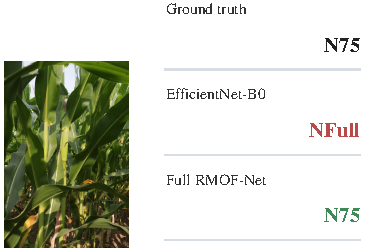
\includegraphics[width=0.92\columnwidth]{figure4_qualitative_case.pdf}
  \caption{Qualitative \Nmid{} diagnostic. The base model predicts \Nfull{}; full \method{} recovers \Nmid{}.}
  \label{fig:case}
\end{figure}

\subsection{Efficiency analysis}

Full \method{} adds 0.303M parameters (7.6\%) to EfficientNet-B0 and remains 61.4\% smaller than ResNet18. As shown in Figure~\ref{fig:cost}, it obtains 0.715 Macro-F1 with 4.314M parameters, compared with 0.588 Macro-F1 and 11.178M parameters for ResNet18. Marker colour and area encode the associated latency: the colour path increases batch-one latency from 0.555 to 1.143 ms/image. The inset shows a non-monotonic response to ECP, followed by larger gains from learned texture and region-wise fusion. Cross-attention increases latency by only 0.006 ms over the scalar-gate variant. Thus, the base model is preferable under a strict latency constraint, whereas \method{} trades latency for improved middle-class and endpoint performance.

\begin{figure}[!t]
  \centering
  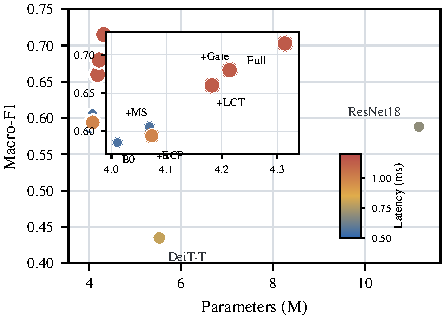
\includegraphics[width=0.88\columnwidth]{figure5_performance_cost.pdf}
  \caption{Performance--cost trade-off. Colour and marker area encode batch-one latency; the inset resolves the EfficientNet component ladder.}
  \label{fig:cost}
\end{figure}

The main panel compares independent baselines with the final model, whereas the inset compares variants that retain the EfficientNet-B0 trunk. Multi-scale regions provide an initial low-cost improvement; explicit priors do not improve all metrics; learned texture produces the larger increase; and region-wise fusion gives the final improvement at almost unchanged parameter count. The gain is accompanied by higher \Nmid{} F1 and fewer endpoint reversals, rather than by a shift toward a single endpoint class.

\subsection{Binary and ordinal outputs}

The binary and ordinal outputs measure distinct aspects of the task. Def.-F1 evaluates whether a canopy differs from the \Nfull{} reference, Macro-F1 weights the three treatment levels equally, and ordinal MAE distinguishes adjacent errors from endpoint reversals. In an inspection workflow, the deficiency score can prioritise images and the ordered label can provide a treatment-level estimate. The improvement in \Nmid{} F1 and reduction in $\pm2$ residuals indicate improved discrimination near the intermediate treatment.

The outputs are not calibrated fertiliser recommendations. The study does not link RGB labels to tissue nitrogen, yield, or fertiliser dose. Any operational use should retain the image and model outputs, record acquisition conditions, and refer unfamiliar or uncertain cases for manual inspection.

\section{Reproducibility and limitations}

For reproducibility, the evaluation should retain split manifests, duplicate clusters, fitted foreground thresholds, colour-standardisation statistics, per-image logits, auxiliary scores, class predictions, and timing repetitions. These records permit regeneration of Table~\ref{tab:main} and Figures~\ref{fig:ablation}--\ref{fig:cost} from a fixed evaluation. Point estimates in the component sequence should be accompanied by matched seeds and paired bootstrap intervals before small differences are treated as stable.

External validation should hold out complete acquisition groups, such as field blocks, dates, cameras, or genotype groups, rather than individual images only. In addition to accuracy, it should report Macro-F1, \Nmid{} F1, ordinal MAE, and endpoint-reversal counts. Stratifying the Figure~\ref{fig:error} analysis by illumination and canopy coverage would test whether the colour stream remains effective under changed image conditions.

The treatment labels are application levels rather than direct tissue-nitrogen measurements. RGB colour also varies with camera, illumination, growth stage, genotype, weeds, and senescence. The present experiment uses one field dataset and does not establish cross-farm transfer. \method{} should therefore be interpreted as an RGB treatment-level classifier, not as a calibrated fertiliser recommendation system. Field trials linked to tissue nitrogen, yield, soil, and weather would be required before operational use.

\section{Conclusion}

\method{} combines multi-scale CNN features, regional colour statistics, learned colour texture, region-wise cross-attention, and ordinal supervision. Relative to EfficientNet-B0, it improves Macro-F1 by 0.130, \Nmid{} F1 by 0.055, and reduces ordinal MAE from 0.535 to 0.310. It also reduces endpoint reversals from 24 to five with a modest parameter increase. The ablation indicates that learned local colour texture and regional fusion contribute to these gains. Validation across independent fields and acquisition conditions remains necessary before using the model for field nitrogen assessment.

\FloatBarrier
\clearpage
\balance
\begin{thebibliography}{99}
\footnotesize

\bibitem{sethy2020}
P. K. Sethy, N. K. Barpanda, A. K. Rath, and S. K. Behera, ``Nitrogen deficiency prediction of rice crop based on convolutional neural network,'' \emph{J. Ambient Intell. Humanized Comput.}, vol. 11, no. 11, pp. 5703--5711, 2020.

\bibitem{salaic2023}
M. Salai\'{c}, F. Novoselnik, I. Podnar \v{Z}arko, and V. Gali\'{c}, ``Nitrogen deficiency in maize: Annotated image classification dataset,'' \emph{Data in Brief}, vol. 50, Art. no. 109625, 2023.

\bibitem{mohanty2016}
S. P. Mohanty, D. P. Hughes, and M. Salath\'{e}, ``Using deep learning for image-based plant disease detection,'' \emph{Frontiers Plant Sci.}, vol. 7, Art. no. 1419, 2016.

\bibitem{plantdoc2020}
D. Singh, N. Jain, P. Jain, P. Kayal, S. Kumawat, and N. Batra, ``PlantDoc: A dataset for visual plant disease detection,'' in \emph{Proc. ACM IKDD CoDS/COMAD}, 2020, pp. 249--253.

\bibitem{mvmatch2024}
J. Yi, Y. Luo, M. Deichmann, G. Schaaf, and J. Gall, ``MV-Match: Multi-view matching for domain-adaptive identification of plant nutrient deficiencies,'' arXiv:2409.00903, 2024.

\bibitem{resnet2016}
K. He, X. Zhang, S. Ren, and J. Sun, ``Deep residual learning for image recognition,'' in \emph{Proc. CVPR}, 2016, pp. 770--778.

\bibitem{efficientnet2019}
M. Tan and Q. V. Le, ``EfficientNet: Rethinking model scaling for convolutional neural networks,'' in \emph{Proc. ICML}, 2019, pp. 6105--6114.

\bibitem{deit2021}
H. Touvron, M. Cord, M. Douze, F. Massa, A. Sablayrolles, and H. J\'{e}gou, ``Training data-efficient image transformers and distillation through attention,'' in \emph{Proc. ICML}, 2021, pp. 10347--10357.

\bibitem{woebbecke1995}
D. M. Woebbecke, G. E. Meyer, K. von Bargen, and D. A. Mortensen, ``Color indices for weed identification under various soil, residue, and lighting conditions,'' \emph{Trans. ASAE}, vol. 38, no. 1, pp. 259--269, 1995.

\bibitem{meyer2008}
G. E. Meyer and J. C. Neto, ``Verification of color vegetation indices for automated crop imaging applications,'' \emph{Comput. Electron. Agric.}, vol. 63, no. 2, pp. 282--293, 2008.

\bibitem{arevalo2017}
J. Arevalo, T. Solorio, M. Montes-y-G\'{o}mez, and F. A. Gonz\'{a}lez, ``Gated multimodal units for information fusion,'' arXiv:1702.01992, 2017.

\bibitem{hou2016}
L. Hou, C.-P. Yu, and D. Samaras, ``Squared Earth Mover's Distance-based loss for training deep neural networks,'' arXiv:1611.05916, 2016.

\bibitem{imagenet2009}
J. Deng, W. Dong, R. Socher, L.-J. Li, K. Li, and L. Fei-Fei, ``ImageNet: A large-scale hierarchical image database,'' in \emph{Proc. CVPR}, 2009, pp. 248--255.

\bibitem{adamw2019}
I. Loshchilov and F. Hutter, ``Decoupled weight decay regularization,'' in \emph{Proc. ICLR}, 2019.

\end{thebibliography}

\end{document}
